\section{Co-Regular of Priority Queues}
\label{sec:co-regular of priority queues}

A rule $R$ of priority queue is co-regular, if checking linearizability with respect to $\textit{MS}(R)$ of a data-independent implementation $\mathcal{I}$ can be reduced to checking the emptiness of intersection between $\mathcal{I}$ and a set of witness automata. In this section, we propose the definition of witness automata and co-regular. Then we prove that all five rules of priority queues are co-regular, and roughly introduce the proof idea. With the help of step-by-step linearizability and co-regular, we finally reduce the linearizability problem of $\textit{PQueue}$ into emptiness problem of intersection with automata.



\subsection{Definition of Co-Regular}
\label{subsec:definition of co-regular}

A witness automaton is a finite automaton with alphabet $\{ \textit{cal}(\textit{put},d,\textit{pre}), \textit{ret}(\textit{put}d),$ $\textit{cal}(\textit{rm},d),\textit{ret}(\textit{rm},d) \vert d \in \mathbb{D},\textit{red} \in \textit{preWA} \}$. Here $\textit{preWA}$ is the set of predicate of priorities, and it contains

\begin{itemize}
\setlength{\itemsep}{0.5pt}
\item[-] A predicate variable $p$, which accepts some specific priority,

\item[-] A predicate $\textit{les}_p$, which accepts all the priorities that are less than the value of $p$,

\item[-] A predicate $\textit{anyPri}$, which accepts any priority.
\end{itemize}

Given a execution $e = \alpha_1 \cdots \alpha_k$ of priority queue and a witness automaton $\mathcal{A}$, we say that $e$ is accepted by $\mathcal{A}$, if

\begin{itemize}
\setlength{\itemsep}{0.5pt}
\item[-] There exist transitions $q_0 \xrightarrow{\beta_1} q_1 \ldots \xrightarrow{\beta_k} q_k$ of $\mathcal{A}$, such that $q_0$ is one of initial state of $\mathcal{A}$, and $q_k$ is one of accept state of $\mathcal{A}$. Let $d_p \in \mathbb{D}$.

\item[-] For each $i$, if $\alpha_i = \textit{cal}(\textit{put},a,q)$, then either (1) $\beta_i = \textit{cal}(\textit{put},a,p)$ and $q = d_p$, or (2) $\beta_i = \textit{cal}(\textit{put},a,\textit{les}_p)$ and $q < d_p$, or (3) $beta_i = \textit{cal}(\textit{put},a,\textit{anyPri})$.

\item[-] For each $i$, if $\alpha_i = \textit{ret}(\textit{put},a)$, or $\alpha_i = \textit{cal}(\textit{rm},a)$, or $\alpha_i = \textit{ret}(\textit{rm},a)$, then $\beta_i = \alpha_i$.
\end{itemize}

Note that witness automata does not read operations, since the domains of operations is infinite.

Let us introduce the notion of co-regular:

%\vspace{-6pt}
\begin{definition}\label{def:co-regular of rules of priority queues}
A rule $R$ of priority queue is co-regular, if there are a finite set $\textit{Auts}_{R}$ of witness automata such that, for each data-independence implementation $\mathcal{I}$, we have that

$$ \textit{Auts}_{R} \cap \mathcal{I} = \emptyset \Leftrightarrow \exists e \in \mathcal{I}_{\neq},e' \in \textit{proj}(e), last(e')=R \wedge e \ does \ not \ linearizable \ w.r.t. \ \textit{MS}(R)$$

We say that $\textit{PQueue}$ is regular, if each of its rule is co-regular.
\end{definition}

Before we go to investigate co-regular of each rules, we use the results in \cite{Bouajjani:2015} to simplify our work. \cite{Bouajjani:2015} states that checking linearizability w.r.t queue can be reduced into checking emptiness of intersection between $\mathcal{I}$ and a set of automata. Given a data-differentiated execution $e$, let $e \vert_{i}$ be an execution generated from $e$ by erasing call and return actions of items that does not use priority $i$. We call a priority queue execution with only one priority a single-priority execution. Let $\textit{transToQueue}(e)$ be an execution generated from $e$ by transforming $\textit{put}$ and $\textit{rm}$ into $\textit{enq}$ and $\textit{deq}$, respectively, and then discarding priorities. We can see that for each $e \in \textit{PQueue}$ and each priority $i$, $\textit{transToQueue}(e \vert_{i})$ satisfy FIFO (first in first out) property.

Given an execution of queue, we say that it is differentiated \cite{Wolper:1986}, if each item is enqueued at most once. \cite{Bouajjani:2015} states that, given a differentiated queue execution $e$ without $\textit{deq}(\textit{empty})$, $e$ is not linearizable with respect to queue, if one of the following cases holds for some $a,b$: (1) $\textit{deq}(b) <_{hb} \textit{enq}(b)$, (2) there are are no $\textit{enq}(b)$ and least one $\textit{deq}(b)$, (3) there are are one $\textit{enq}(b)$ and more than one $\textit{deq}(b)$, and (4) $\textit{enq}(a) <_{\textit{hb}} \textit{enq}(b)$, and $\textit{deq}(b) <_{\textit{hb}} \textit{deq}(a)$, or $\textit{deq}(a)$ does not exists. For each such case, we can construct a witness automata for priority queue. For example, for the first case, we generate witness automata $\mathcal{A}_{\textit{SinPri}}^1$ in \figurename~\ref{fig:automata for FIFO-1}, here $c_1 = \textit{cal}(\textit{put},a,\textit{anyPri}), \textit{ret}(\textit{put},a), \textit{cal}(\textit{rm},a)$, $\textit{ret}(\textit{rm},a),\textit{cal}(\textit{rm},b)$, $c_2 = c_1 + \textit{ret}(\textit{rm},b)$, $c_3 = c_2 + \textit{ret}(\textit{put},b)$.


\begin{figure}[htbp]
  \centering
  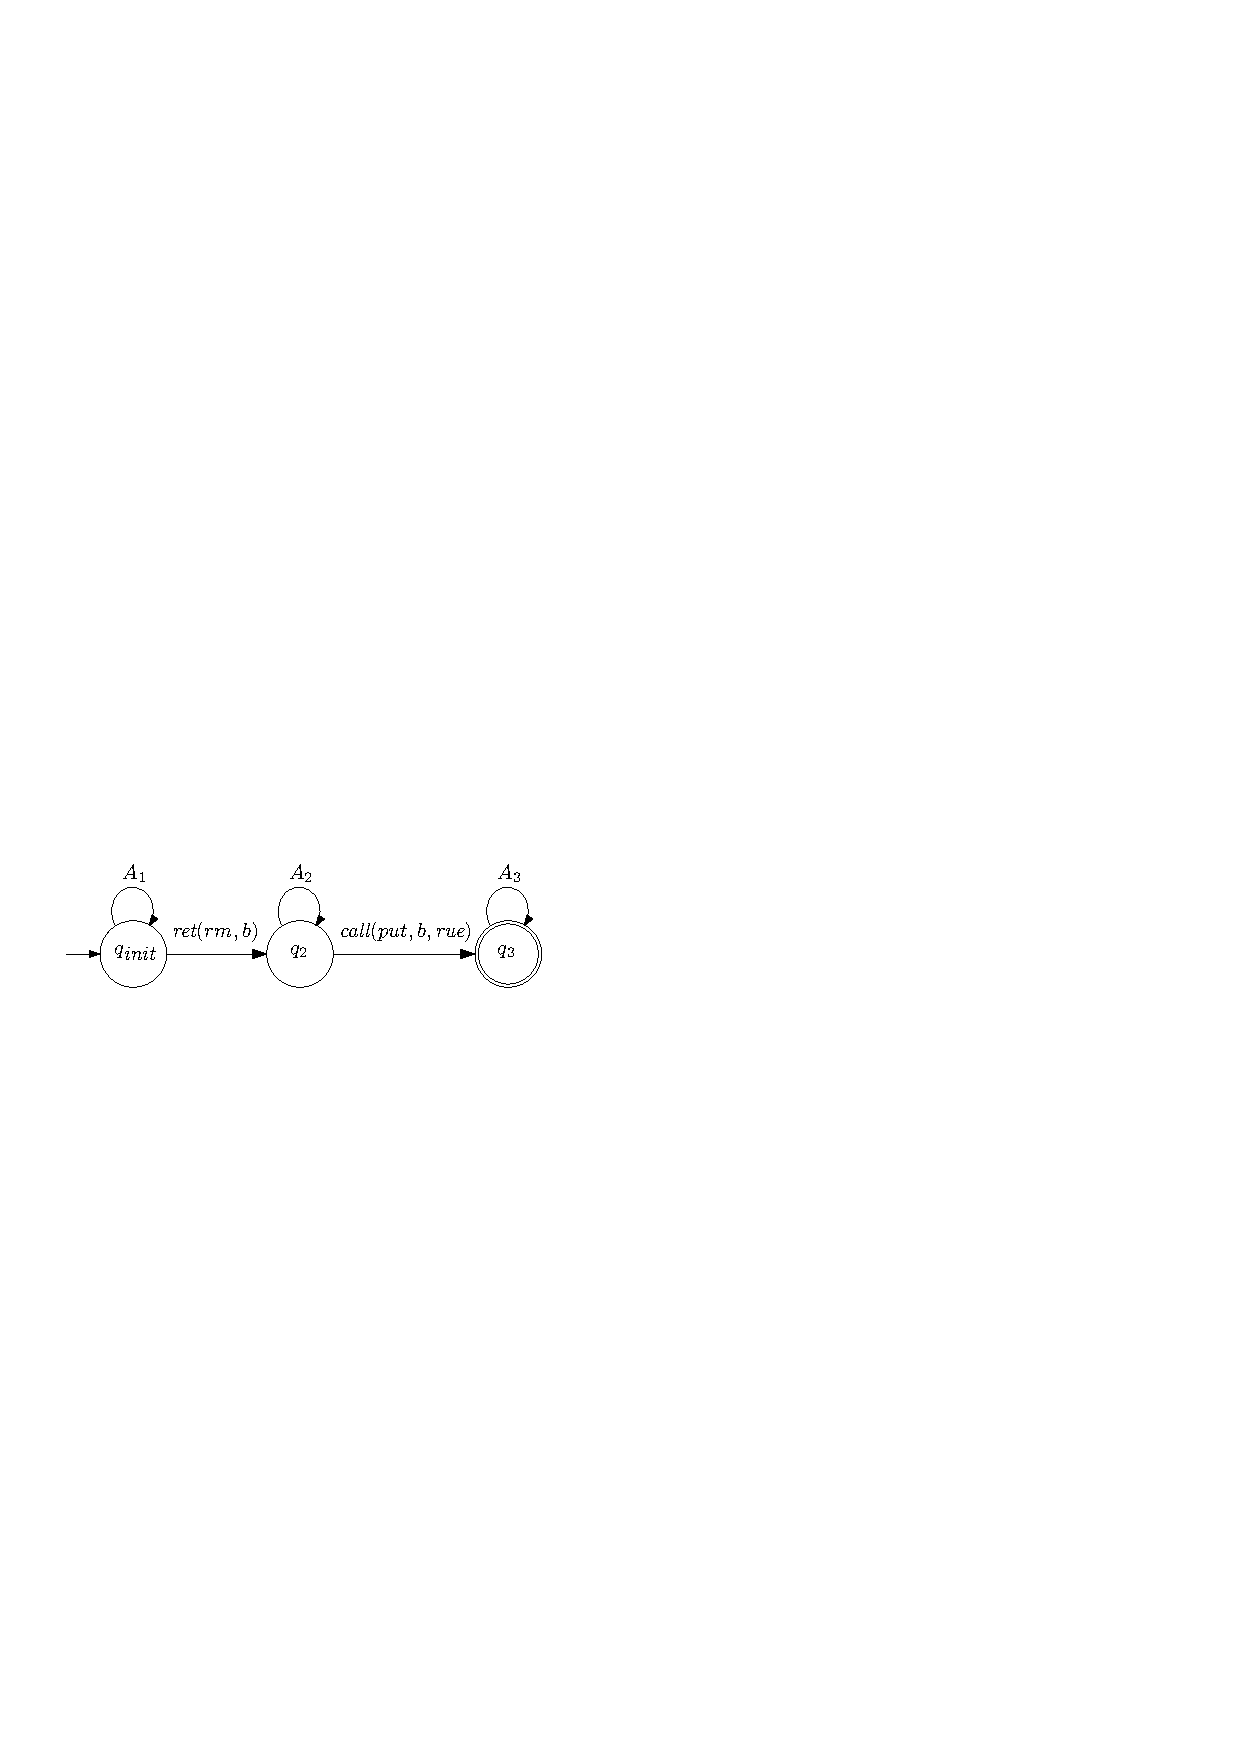
\includegraphics[width=0.6 \textwidth]{figures/PIC_AUTO_FIFO_1.pdf}
%\vspace{-10pt}
  \caption{Automaton $\mathcal{A}_{\textit{SinPri}}^1$}
  \label{fig:automata for FIFO-1}
\end{figure}

In Appendix \ref{sec:appendix proof and definition in section definition of co-regular}, we construct a set $\textit{Auts}_{\textit{sinPri}}$ of witness automata ($\mathcal{A}_{\textit{SinPri}}^1$ is in it), and shows that they are enough to ensure that for each of its data-differentiated executions, each of its single-priority projection that has no $\textit{rm}(\textit{empty})$ to have ``FIFO'' property, as shown by the following lemma.

\begin{restatable}{lemma}{AutoForPQwithSignlePri}
\label{lemma:automata for priority queue with single priority}

Given a data-independent implementations $\mathcal{I}$ of priority queue, $\mathcal{I} \cap \textit{Auts}_{\textit{sinPri}} \neq \emptyset$, if and only if there exists $e \in \mathcal{I}_{\neq}$, $e' \in \textit{proj}(e)$, such that $e'$ is single-priority  without $\textit{rm}(\textit{empty})$, and $\textit{transToQueue}(e')$ does not linearizable to queue.
\end{restatable}

According to Lemma \ref{lemma:automata for priority queue with single priority}, from now on, it is safe to assume that, for each data-differentiated execution without $\textit{rm}(\textit{empty})$, any of its single-priority projection has ``FIFO'' property. For example, $\textit{rm}(a)$ never happens before $\textit{put}(a,\_)$ for each $a$.



\subsection{Co-Regular of $\textit{PQ}_1^{>}$}
\label{subsec:co-regular of PQ1Lar}

In this subsection, we introduce the idea for proving co-regular of $\textit{PQ}_1^{>}$. The proof of this subsection can be found in Appendix \ref{sec:appendix proof and definition in section co-regular of PQ1Lar}. The notion of left-right constraint used for priority queue is inspired by left-right constraint of queue \cite{Bouajjani:2015}.

Given a data-differentiated execution $e$ such that $\textit{last}(e) = \textit{PQ}_1^{>}$, although Lemma \ref{lemma:automata for priority queue with single priority} ensures that each single-priority projection of $e$ satisfy the FIFO property, this is still not enough for ensuring that $e \sqsubseteq \textit{MS}(\textit{PQ}_1^{>})$. Since it is possible that $e$ does not linearizable w.r.t $\textit{MS}(\textit{PQ}_1^{>})$ because of interaction between actions of multiple priorities.

We give an example of such execution $e$ in \figurename~\ref{fig:introduce gap for PQ1Lar}. We call the time interval from $\textit{ret}(\textit{put},x)$ to $\textit{cal}(rm,x)$, or from $\textit{ret}(\textit{put},x)$ when $\textit{cal}(rm,x)$ does not exist, the interval of item $x$. In \figurename~\ref{fig:introduce gap for PQ1Lar}, we draw the interval of each item by dashed line. The reason of why $e$ does not linearizable w.r.t $\textit{MS}(\textit{PQ}_1^{>})$ is that, each time point from $\textit{cal}(\textit{rm},b)$ to $\textit{ret}(\textit{rm},b)$ is in interval of some item with less priority than priority of $a$.

\begin{figure}[htbp]
  \centering
  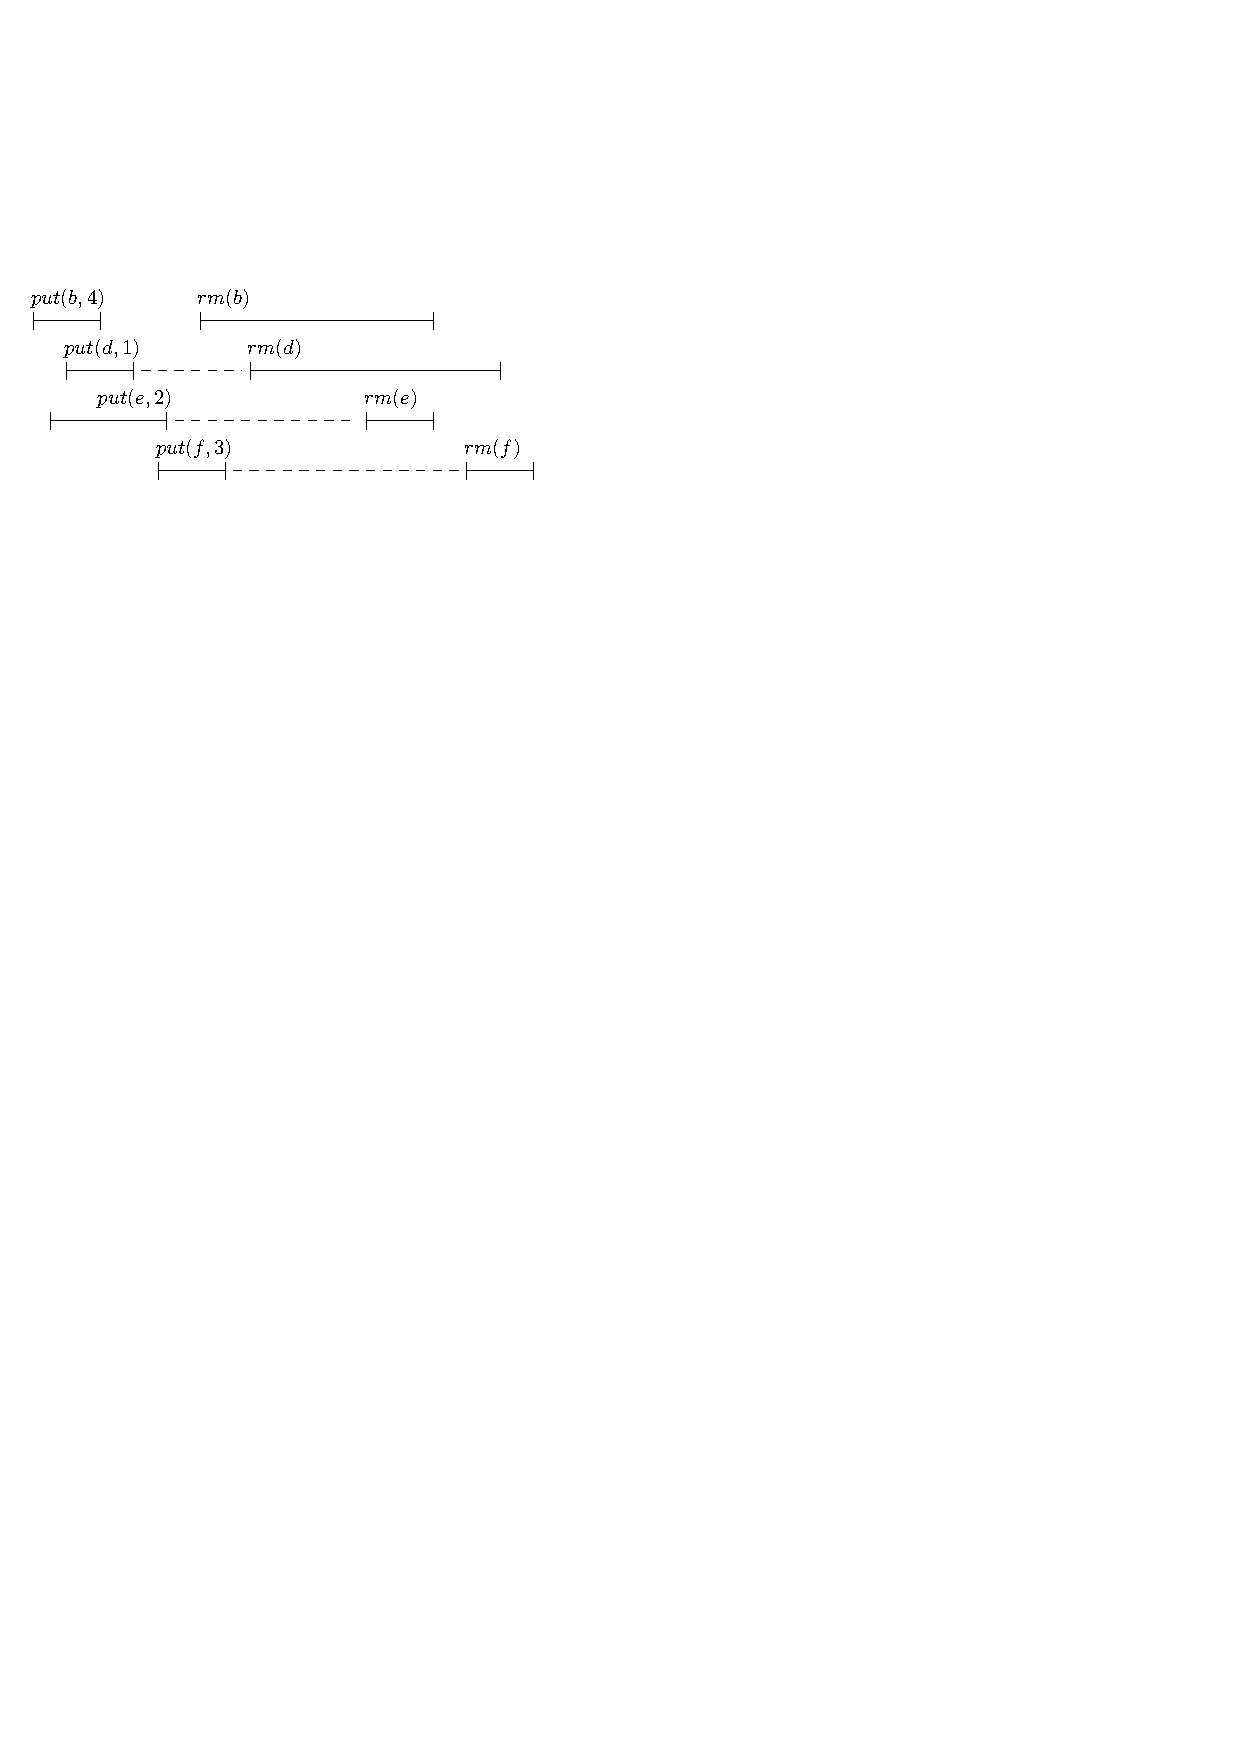
\includegraphics[width=0.6 \textwidth]{figures/PIC-HIS-INTRO-GAP-PQ1L.pdf}
%\vspace{-10pt}
  \caption{An execution that does not linearizable w.r.t $\textit{MS}(\textit{PQ}_1^{>})$}
  \label{fig:introduce gap for PQ1Lar}
\end{figure}

In this subsection, intuitively we will prove that, as long as we can get rid of the case in \figurename~\ref{fig:introduce gap for PQ1Lar}, we can ensure $\textit{last}(e) = \textit{PQ}_1^{>} \Rightarrow e \sqsubseteq \textit{MS}(\textit{PQ}_1^{>})$.

Let us introduce the notion of left-right constraint, which is a graph, and the existence of cycle though item with maximal priority in it correspond to the existence of the case in \figurename~\ref{fig:introduce gap for PQ1Lar}.

\begin{definition}\label{def:left-right constraint for matched put and rm operations}
Given a data-differentiated execution $e$ without $\textit{rm}(\textit{empty})$. Let $\textit{put}(x,\textit{pri}_x)$ and $\textit{rm}(x)$ be method events of $e$, where $\textit{pri}_x$ is maximal in $e$ and only used by these two method events. The left-right constraint of $\textit{put}(x,\textit{pri}_x)$ and $\textit{rm}(x)$ is the graph $G$ where:

\begin{itemize}
\setlength{\itemsep}{0.5pt}
\item[-] the nodes are the items of $e$, to which we add a node,

\item[-] there is an edge from item $d_1$ to $x$, if $\textit{put}(d_1,\textit{pri}_1)$ happens before $\textit{put}(x,\textit{pri}_x)$ or $\textit{rm}(x)$,

\item[-] there is an edge from $x$ to item $d_1$, if $\textit{rm}(x)$ happens before $\textit{rm}(d_1)$ or $\textit{rm}(d_1)$ does not exists in $h$,

\item[-] there is an edge from item $d_1$ to item $d_2$, if $\textit{put}(d_1,\textit{pri}_1)$ happens before $\textit{rm}(d_2,\textit{pri}_2)$.
\end{itemize}
\end{definition}

When there is a cycle $d_1 \rightarrow \ldots \rightarrow d_m \rightarrow x \rightarrow d_1$ through item with maximal priority (for example, $x$) in $G$, we say that $x$ is covered by $d_1,\ldots,d_m$. To state the effectiveness of left-right constraint, take the execution in \figurename~\ref{fig:introduce gap for PQ1Lar} as an example, we can see that $b$ is covered by $f,e,d$. We need to prove that getting rid of cycle though item with maximal priority in left-right constraint is enough for ensure linearizable w.r.t $\textit{MS}(\textit{PQ}_1^{>})$, as stated by the following lemma:

\begin{restatable}{lemma}{LinEqualsConstraintforPQOneLar}
\label{lemma:Lin Equals Constraint for PQ1Lar}
Given a data-differentiated execution $e$ with $\textit{last}(e) = \textit{PQ}_1^{>}$. Let $\textit{put}(x,\textit{pri}_x)$ and $\textit{rm}(x)$ be method events of $e$ with maximal priority. Let $G$ be the graph representing the left-right constraint of $\textit{put}(x)$ and $\textit{rm}(x)$. $e \sqsubseteq \textit{MS}(\textit{PQ}_1^{>})$, if and only if $G$ has no cycle going through $x$.
\end{restatable}

\begin {proof} (Sketch)

The $\textit{only if}$ direction can be easily proved by contradiction and is omitted here. To prove the $\textit{if}$ direction, we need to explicitly construct the linearization of $e$, or we can say, we need construct the $u$, $v$ and $w$ in $\textit{PQ}_1^{>}$. Let $u$ to be the sequence of all operations that happens before $\textit{put}(x)$. The difficulties is how to generate proper $v$.

To generate $v$, we introduce $\textit{UVSet}(e,x)$, which intuitively contains all pairs of method events that should be putted before $\textit{rm}(x)$. Let $\textit{UVSet}_1(e,x)= \{ o \vert$ either $o <_{\textit{hb}} \textit{put}(x)$ or $\textit{rm}(x)$, or $\exists o'$ with the same item of $o$, such that $o' <_{\textit{hb}} \textit{put}(x)$ or $\textit{rm}(x)\}$. For each $i \geq 1$, let $\textit{LMSet}_{\textit{i+1}}(e,x) = \{ o \vert$ $o \notin \textit{UVSet}_k(e,x)$ for each $k \leq i$, and either $o$ happens before some operation $o' \in \textit{UVSet}_i(e,x)$, or $\exists o''$ with the same item of $o$ and $o''$ happens before some operation $o' \in \textit{UVSet}_i(e,x)\}$. Let $\textit{UVSet}(e,x) = \textit{UVSet}_1(e,x) \cup \textit{UVSet}_2(e,x) \cup \ldots$. For example, in \figurename~\ref{fig:his nobound of LMSet}, $\textit{UVSet}_1(e,x) = \{ \textit{put}(a,1),\textit{rm}(a) \}$, $\textit{USSet}_2(e,x) = \{ \textit{put}(b,1),\textit{rm}(b) \}$ and $\textit{UVSet}_3(e,x) = \{ \textit{put}(a,c),\textit{rm}(c) \}$. Similarly, we can generate execution $e'$ such that, for each $i$, $\textit{UVSet}(e',x) \neq \emptyset$.


\begin{figure}[htbp]
  \centering
  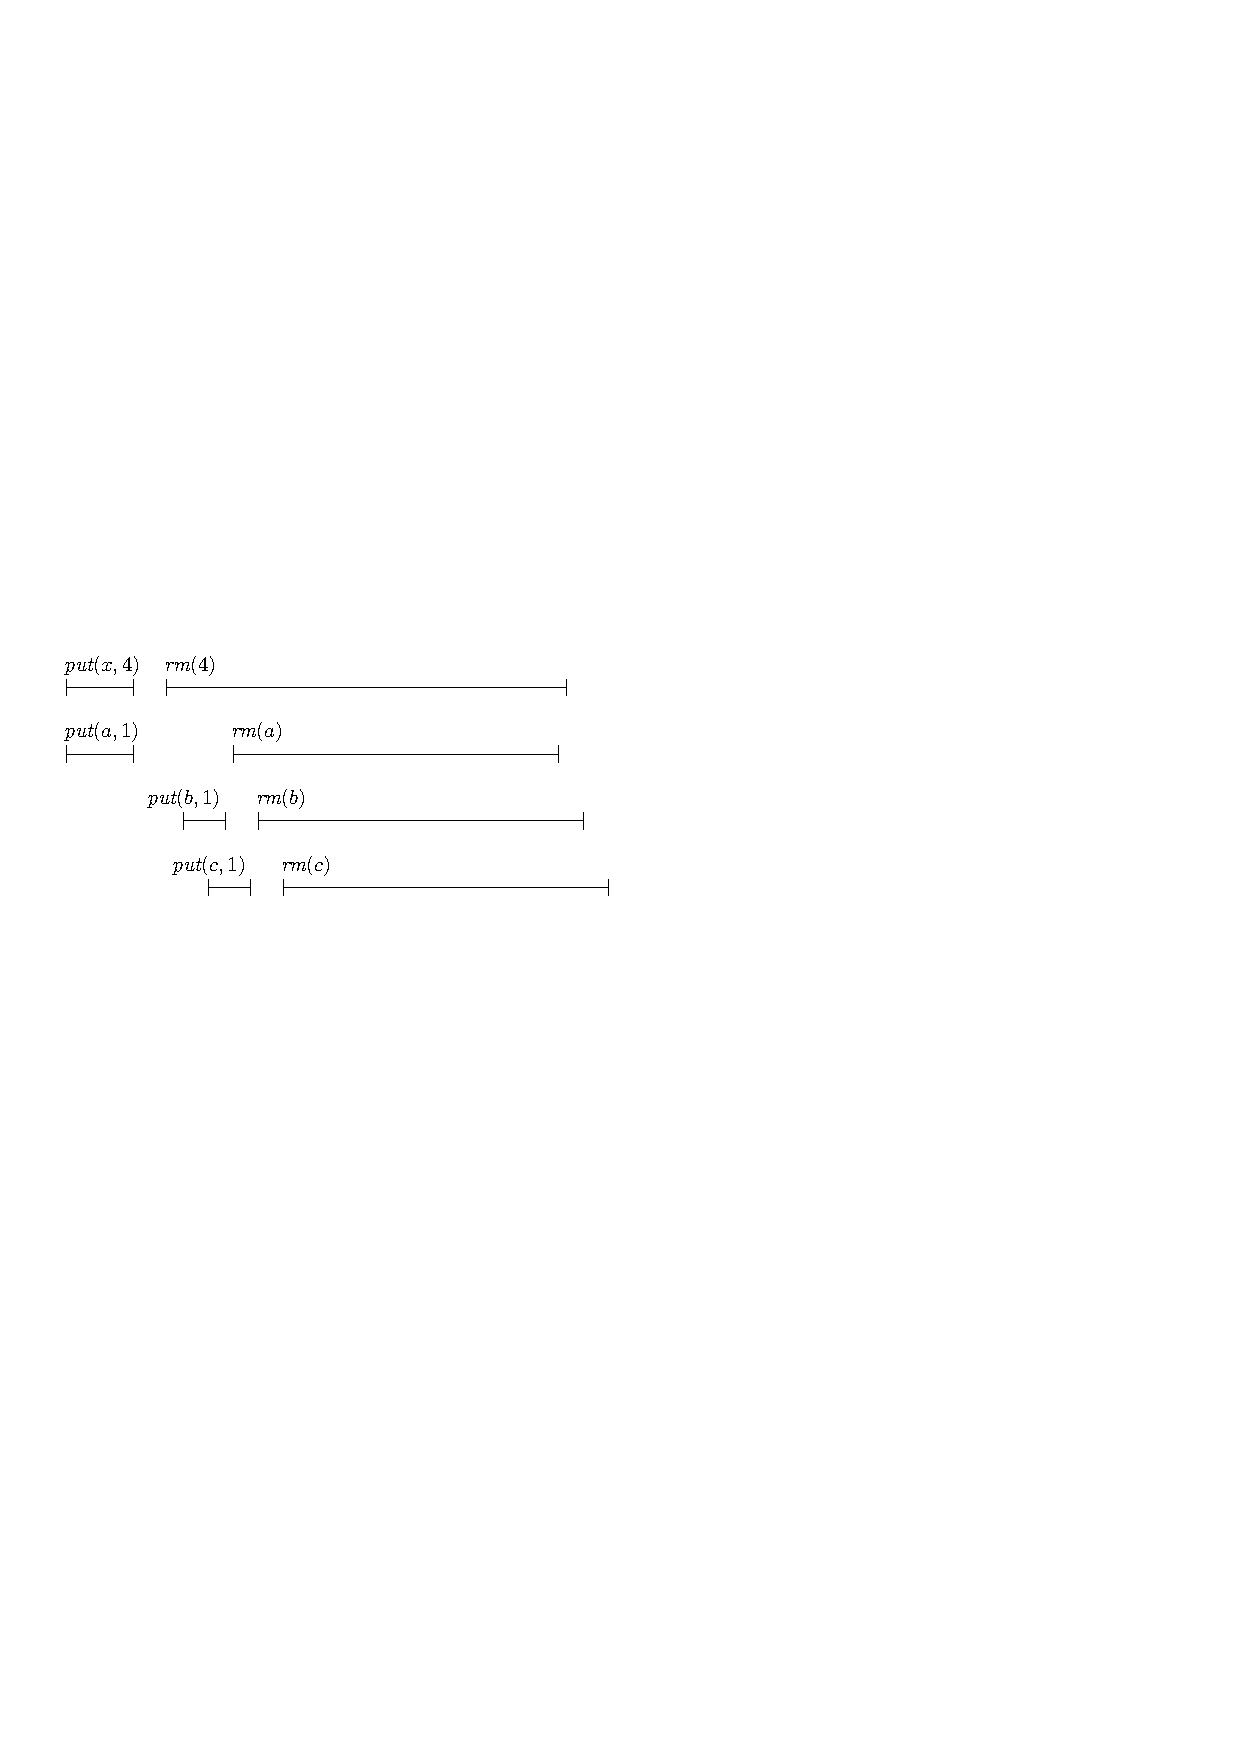
\includegraphics[width=0.5 \textwidth]{figures/PIC_HIS_NOBOUNDOF_LMSET.pdf}
%\vspace{-10pt}
  \caption{An example for $\textit{UVSet}(e,x)$}
  \label{fig:his nobound of LMSet}
\end{figure}

We let the $v$ to be the sequence of method events that are in $\textit{UVSet}(e,x)$ and not in $u$. We let $w$ to be the sequence of remaining method events. Then we can prove that such $u$, $v$ and $w$ holds as required. \qed
\end {proof}

According to Lemma \ref{lemma:Lin Equals Constraint for PQ1Lar}, the existence of ``cover item with maximal priority'' is enough for checking violation of linearizability w.r.t $\textit{MS}(\textit{PQ}_1^{>})$. Assume $x$ is covered by $d_1,\ldots,d_m$. Then we can safely rename $x$ into $b$, rename $d_1,\ldots,d_m$ into $a$ and rename all other item into $c$ by data-independence. Such execution can be recognized by witness automata, since between the first $\textit{ret}(\textit{put},a,\_)$ and the last $\textit{cal}(\textit{rm},a)$ (if exists), $\textit{ret}(\textit{put},a,\_)$ and $\textit{cal}(\textit{rm},a)$ occurs in pair and there is no need for count.

There are four possible enumeration of call and return actions of $\textit{put}(b)$ and $\textit{rm}(b)$. For each of them, we generate a witness automaton. For example, for the case when $e \vert_{b} = \textit{cal}(\textit{put},b,p) \cdot \textit{ret}(\textit{put}) \cdot \textit{cal}(\textit{rm}) \cdot \textit{ret}(\textit{rm},b)$, we generate witness automaton $\mathcal{A}_{\textit{l-lar}}^1$, as shown in \figurename~\ref{fig:automata APQ1Lar-1}. Here $c_1 = c + \textit{ret}(\textit{rm},a)$, $c_2 = c + \textit{cal}(\textit{put},a,\textit{les}_p)$, $c_3 = c_2 + \textit{ret}(\textit{rm},a)$, where $c = \textit{cal}(\textit{put},d,\textit{anyPri}),\textit{ret}(\textit{put},d), \textit{cal}(\textit{rm},d), \textit{ret}(\textit{rm},d)$.

\begin{figure}[htbp]
  \centering
  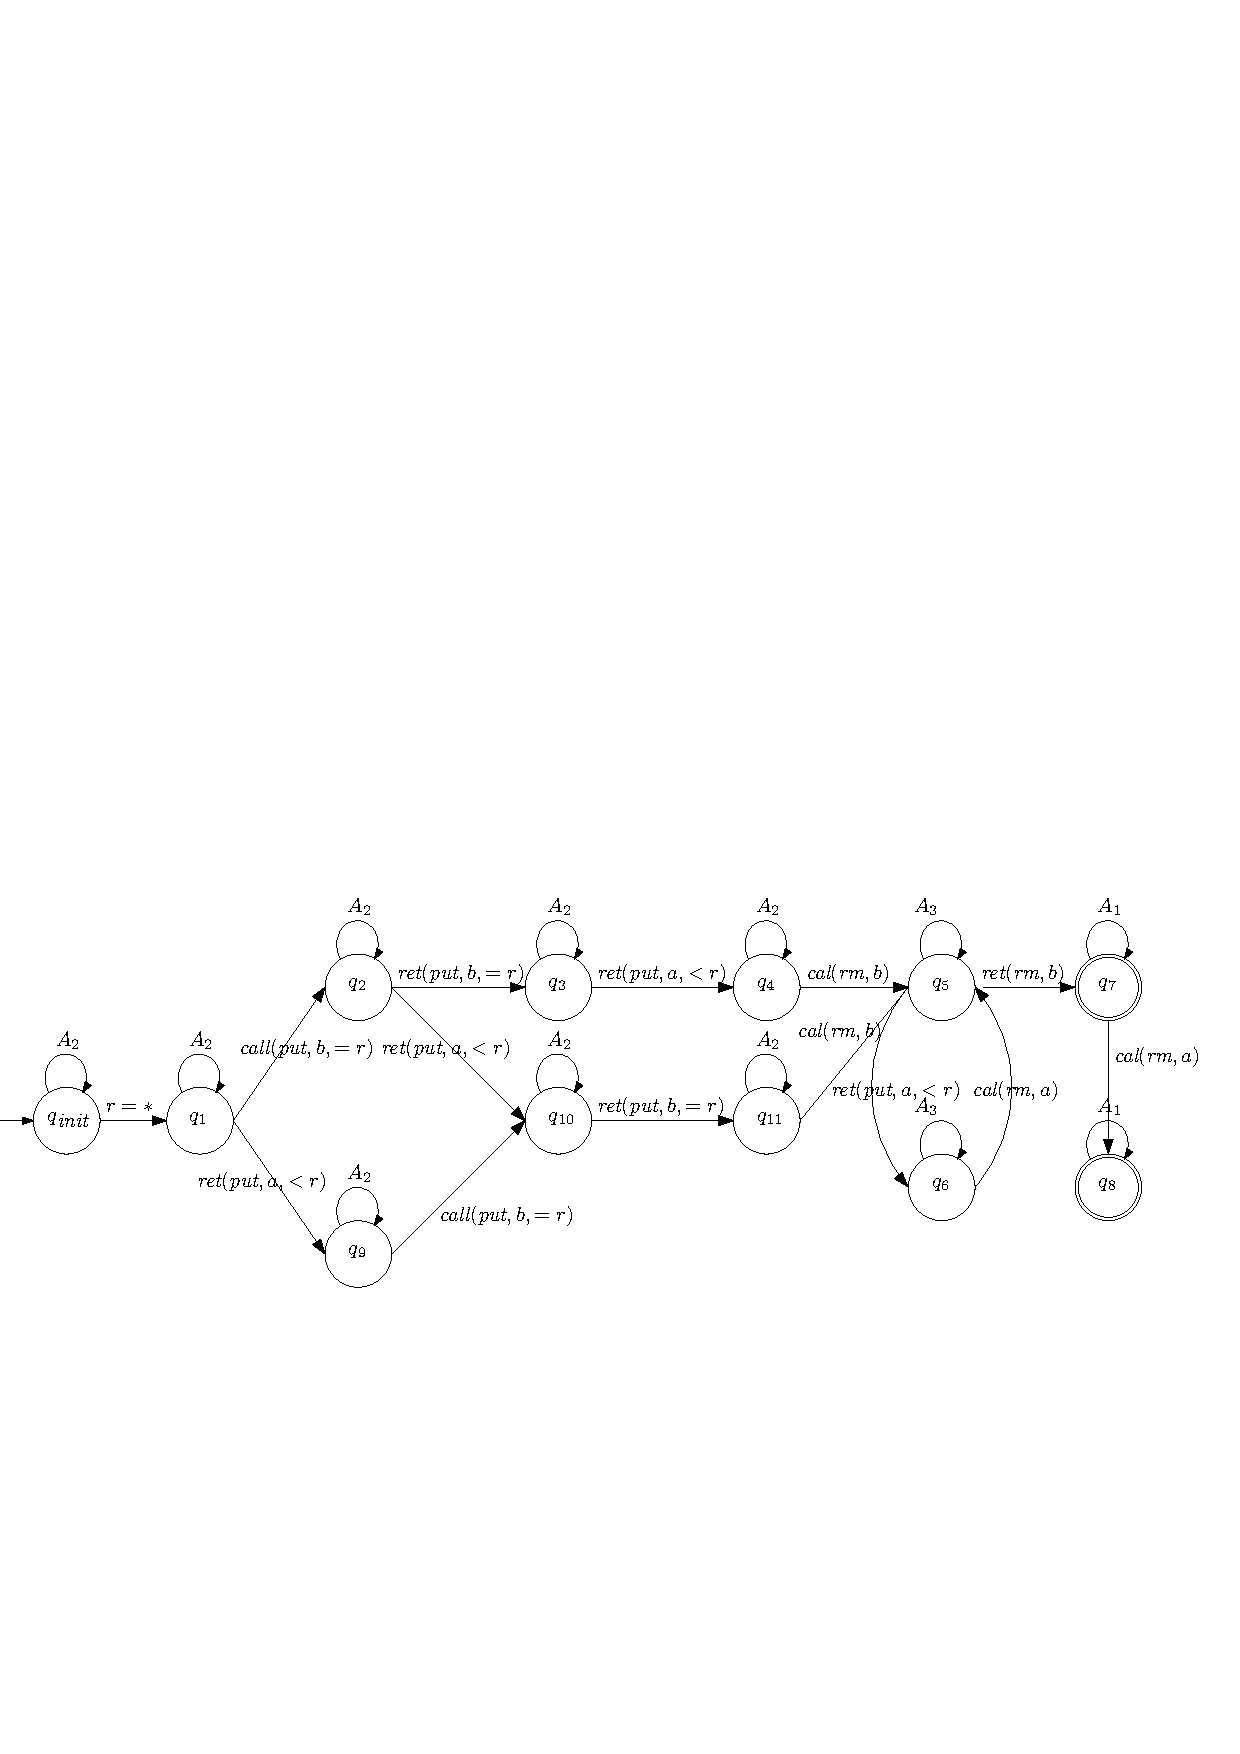
\includegraphics[width=1 \textwidth]{figures/PIC_AUTO_PQ1Lar-pprr.pdf}
%\vspace{-10pt}
  \caption{Automaton $\mathcal{A}_{\textit{l-lar}}^1$}
  \label{fig:automata APQ1Lar-1}
\end{figure}

Given the execution $e$ in \figurename~\ref{fig:introduce gap for PQ1Lar}, let $e'$ be generated from $e$ by renaming $d,e,f$ into $a$. Then we can see that $e'$ is accepted by $\mathcal{A}_{\textit{l-lar}}^1$ with a path via $q_{\textit{init}}, q_2, q_3, q_4,q_5,q_7,q_8$.

In Appendix \ref{sec:appendix proof and definition in section co-regular of PQ1Lar}, we construct a set $\textit{Auts}_{\textit{1-lar}}$ of witness automata ($\mathcal{A}_{\textit{l-lar}}^1$ is in it), and use $\textit{Auts}_{\textit{1-lar}}$ to prove that $\textit{PQ}_1^{>}$ is co-regular, as stated by the following lemma.

\begin{restatable}{lemma}{PQOneLarisCoRegular}
\label{lemma:PQ1Lar is co-regular}
$\textit{PQ}_1^{>}$ is co-regular.
\end{restatable}










